The last trick for our bag to embark on the KFAC journey is linearization.
It is a useful tool whenever we encounter a composition of functions that we would like to convexify.

Consider for example the function $f = g \circ h$ with $f,g,h: \sR \to \sR$ for simplicity.
We know that convexity is preserved under function composition, so if both $g$ and $h$ are convex, then $f$ will be convex.
But what if only one of the two composites is convex, lets say $g$, but $h$ is not?
Well, then we can replace $h$ with an approximation $h'$ that is convex and approximates the original function somewhat well.
Let's say we are interested in only a neighbourhood around $\vx_0$.
Then, we can obtain a simple, convexified approximation $f' \approx f$ in that neighbourhood by linearizing $h$ around $\vx_0$, resulting in a function $(\lin_{\vx_0}(h))(\vx)$.
This involves a first-order Taylor approximation:

\switchcolumn[1]*
\codeblock{linearization}
\switchcolumn[0]

\begin{definition}[Linearization (vector case)]\label{def:vector_linearization}
  Consider a vector-to-vector function $f: \sR^A \to \sR^B, \va \mapsto \vb = f(\va)$.
  The linearization of $f$ at an anchor point $\va_0 \in \sR^A$ denoted by $\lin_{\va_0}(f): \sR^A \to \sR^B$ is its first-order Taylor expansion,
  \begin{align*}
    (\lin_{\va_0}(f))(\va) = f(\va_0) + \jac_{\va_0}f(\va_0) (\va - \va_0)\,,
  \end{align*}
  with the Jacobian from \Cref{def:vector_jacobian}.
  Note that $\lin_{\va_0}(f)$ is linear in $\va$ and coincides with the original function at the anchor point, $(\lin_{\va_0}(f))(\va_0) = f(\va_0)$ (also the Jacobian does).
\end{definition}

\begin{definition}[Linearization (tensor case, \Cref{linearization})]\label{def:tensor_linearization}
  The linearization of a tensor-to-tensor function from \Cref{setup:jacobians} at an anchor point $\tA_0 \in \sR^{A_1 \times \ldots \times A_N}$, denoted by $\lin_{\tA_0}(f)$ is defined per-entry as
  \begin{align*}
    \left[
    (\lin_{\tA_0}(f))(\tA)
    \right]_{j_1, \ldots, j_M}
    = f(\tA_0)
    \\
    +
    \sum_{i_1, \ldots, i_N}
    \left[
    \jac_{\tA_0}f(\tA_0)
    \right]_{j_1, \ldots, j_M, i_1, \ldots, i_N}
    \\
    \left[
    \tA - \tA_0
    \right]_{i_1, \ldots, i_N}\,,
  \end{align*}
  with the Jacobian from \Cref{def:general_jacobian}. Note that this is nothing else but the function evaluated at the anchor point plus the JVP (\Cref{def:jvp}) with the distance to the anchor.
\end{definition}

In deep learning, we will often face the situation where $f = g \circ h, \tA \mapsto b = f(\tA)$ and $h$ is non-convex while $g$ is convex.
This means the Hessian of $f$ can be indefinite; but for algorithms we require a positive definite approximation to the Hessian.
We can obtain that by considering the partially linearized function $f' = g \circ \lin_{\tA_0}(h)$, whose Hessian is positive semi-definite. The Hessian of this partially linearized function is called the generalized Gauss-newton (GGN) matrix.

Let's stick to our one-dimensional example for a moment, i.e.\,let $f(x) = (g \circ h)(x) \in \sR$. If we use the chain rule twice, we obtain the following expression for the Hessian:
\begin{align*}
  \hess_x (g \circ h)(x) =
  \jac_x h(x) \cdot \hess_{h(x)} g(h(x)) \cdot \jac_x h(x)
  \\
  +
  \hess_x h(x) \cdot \jac_{h(x)} g(h(x))\,.
\end{align*}
Now, if we take the hessian of the partially linearized function $f'(x) = (g \circ \lin_{x_0}(h))(x)$, and using the shorthand $h' = \lin_{x_0}(h)$ the second term disappears as the linear function's Hessian is zero:
\begin{align*}
  \hess_x (g \circ h')(x) =
  \jac_x h'(x) \cdot \hess_{h'(x)} g(h'(x)) \cdot \jac_x h'(x)
  \\
  +
  \underbrace{\hess_x h'(x)}_{= 0} \cdot \jac_{h'(x)} g(h'(x))\,.
\end{align*}
If we evaluate both equations at the anchor point, setting $x = x_0$, we obtain that the first terms coincide.

We will not use the linearization aspect explicitly in the computation, but instead rely on GGN-vector products.

TODO Vector case

\begin{definition}[Generalized Gauss-Newton (GGN) tensor (\Cref{ggns}]
  Let $f = g \circ h$ be a tensor-to-scalar function via an intermediate tensor, $f: \sR^{A_1 \times \ldots \times A_N} \to \sR$ with intermediate $h: \sR^{A_1 \times \ldots \times A_N} \to \sR^{B_1 \times \ldots \times B_M}$.
  The generalized Gauss-newton (GGN) tensor $\ggn_x f(\tA) \in \sR^{A_1 \times  \ldots \times A_N \times A_1 \times \ldots \times A_N}$ is the Hessian of the partially linearized function $f' = g \circ \lin_{\tA_0}(h)$, evaluated at the anchor point $\tA_0 = \tA$.
  \begin{align*}
    \tG_{\tA} f(\tA)
    =
    \hess_{\tA} \tilde{f}(\tA)|_{\tA_0 = \tA}\,.
  \end{align*}
  where $\tilde{f} = g \circ \lin_{\tA_0}(h)$
\end{definition}

TODO Flattened GGNs

It is easy to see that $\ggn^{\vec} = {\jac^{\vec}}^{\top} \hess^{\vec} \jac^{\vec}$ where $\vec$ is one of the flattening operations from \Cref{def:cvec,def:rvec}.


\switchcolumn[1]*
\codeblock{ggn_rosenbrock}
\switchcolumn[0]

\begin{example}[GGN for the Rosenbrock function, \Cref{ggn_rosenbrock}]
  Consider the 2d Rosenbrock function $f_{\alpha}: \sR^2 \to \sR$ with
  \begin{align*}
    f_{\alpha}(\vx)
    =
    (1 - x_1)^2 + \alpha (x_2 - x_1^2)^2\,.
  \end{align*}
  with some $\alpha > 0$.
  We can express $f_{\alpha} = \ell \circ g_{\alpha}$,\footnote{\url{https://www.brnt.eu/phd/node10.html}}
  \begin{align*}
    g_{\alpha}(\vx) = \begin{pmatrix}
                        x_1 \\
                        \sqrt{\alpha} (x_2 - x_1^2)
                      \end{pmatrix}
    \shortintertext{and convex}
    \ell(\vg) = \vg^\top \vg\,,
  \end{align*}
  namely square loss.

  Linearizing $g_{\alpha}$ w.r.t. $\vx$ around $\vx'$ gives
  \begin{align*}
    g^{\text{lin}}_{\alpha}(\vx) = g_{\alpha}(\vx') + (\jac_{\vx'}g_{\alpha}(\vx')) (\vx - \vx')\,.
  \end{align*}
  with
  \begin{align*}
    \jac_{\vx}g_{\alpha}(\vx)
    =
    \begin{pmatrix}
      1 & 0 \\
      -2 \sqrt{\alpha} x_1 & \sqrt{\alpha}
    \end{pmatrix}\,.
  \end{align*}
  The first way to form the Hessian is to take the Hessian of $f_{\alpha}' = \ell \circ g_{\alpha}^{\text{lin}}$, and evaluate it at $\vx' = \vx$,
  \begin{align*}
    (\hess_{\vx} f_{\alpha}'(\vx))|_{x=x'}
    \\
    =
    2 (\jac_{\vx} g_{\alpha}(\vx))|_{x=x'}^{\top}
    (\jac_{\vx} g_{\alpha}(\vx))|_{x=x'}
    \\
    =
    2
    \begin{pmatrix}
      1 + 4\alpha x_1^2& -2 \sqrt{\alpha} x_1\\
      -2 \sqrt{\alpha} x_1 & \alpha
    \end{pmatrix}
  \end{align*}
  This matrix is PSD because it is an outer product of two matrices.
  It is also different from the Hessian matrix
  \begin{align*}
    \hess_{\vx} f_{\alpha}(\vx)
    =
    \begin{pmatrix}
      2 + 12 \alpha x_1^2 - 4 \alpha x_2 & -4 \alpha x_1 \\
      -4 \alpha x_1 & 2 \alpha
    \end{pmatrix}
  \end{align*}
  \begin{figure}[H]
    \centering
    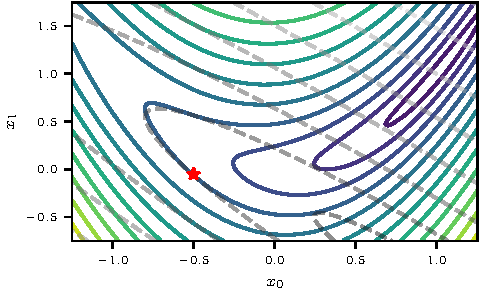
\includegraphics[width=\linewidth]{../kfs/plots/linearized_rosenbrock.pdf}
    \caption{The 2d Rosenbrock function $f_{\alpha=10}$ (solid contour lines) with and its approximation $f'_{\alpha=10, \vx'} = \ell \circ g^{\text{lin}}_{\alpha=10, \vx'}$ (dashed contour lines) when partially linearizing it around an anchor $\vx'$ (star).}
  \end{figure}
\end{example}

%%% Local Variables:
%%% mode: latex
%%% TeX-master: "../main"
%%% End:
